\documentclass[11pt]{article}

\usepackage[margin=1in]{geometry}
\usepackage{amsmath,amssymb}
\usepackage{booktabs}
\usepackage{graphicx}
\usepackage{microtype}
\usepackage[numbers,sort&compress]{natbib}
\usepackage[colorlinks=true,citecolor=blue,linkcolor=blue,urlcolor=blue]{hyperref}
\emergencystretch=2em

\title{Population Digital Red Queen:\\A Model of LLM-Driven Coevolution in Program Ecosystems}
\author{Gabriel Kahen}
\date{May 22, 2026}

\begin{document}
\maketitle

\begin{abstract}
Digital Red Queen (DRQ) reframes LLM-based program synthesis as adversarial adaptation: each new Core War warrior is generated to defeat previously discovered warriors, producing a lineage shaped by its own history. This paper asks whether the process changes when the unit of adaptation is a population rather than a single champion. We introduce Population Digital Red Queen (PDRQ), a family of LLM-driven coevolutionary algorithms that maintain simultaneous programs, sample live and historical opponents, and use archive pressure and niche-preserving replacement to search for robust or complementary strategies. Finite-game examples show why populations can matter in non-transitive adversarial domains, but also why population structure is not automatically beneficial: specialists help only under the right evaluation and deployment assumptions. We test this distinction in a matched-budget Core War study using Gemini 2.5 Flash to generate Redcode warriors. Across 40 long-profile runs, archive+niche PDRQ does not improve mean final-population performance; linear DRQ has the highest observed mean on that metric. Archive+niche PDRQ does, however, produce the highest average best-champion score, with a paired advantage of about 0.06 held-out score over both baselines and bootstrap support of 97.7\% for having the highest mean best-champion score among the tested methods. External replay against Wilkies, WilMoo, Koenigstuhl 94nop, and CGM1 benchmarks is negative: the generated champions are not claimed to be hill-competitive. The result is therefore deliberately narrow: archive+niche pressure is useful as a search-diversification mechanism for finding high-performing outliers inside this controlled evaluation, not as evidence of broad population-level dominance or competitive Core War strength.
\end{abstract}

\section{Introduction}

Large language models have made program synthesis usable as a mutation operator: they can repair code, recombine examples, and generate semantically meaningful variants that are difficult to obtain from character-level or syntax-level mutation alone. Recent systems exploit this ability for open-ended discovery, including FunSearch-style program search \citep{romeraparedes2024funsearch}, evolution through large models \citep{lehman2022elm}, language-model crossover \citep{meyerson2024lmx}, and LLM-assisted architecture search \citep{liu2023evoprompting}. Most such systems, however, still optimize against a fixed objective or a fixed evaluation distribution.

Digital Red Queen (DRQ) changes the objective itself. In the Core War setting, an LLM repeatedly generates a new warrior to defeat the set of previous warriors, producing an adversarial lineage rather than a static hill climb \citep{kumar2026digital}. Prior DRQ results report improved generalization against held-out human warriors and behavioral convergence across independent runs. That convergence suggests that linear self-play can discover robust generalist strategies under the tested evaluation distribution.

But a single champion lineage is only one way to model adversarial adaptation. Biological Red Queen dynamics are population processes: fitness depends on the frequency of other types, specialists can persist when their prey are common, and ecosystems can cycle or branch rather than converge to a single winner \citep{vanvalen1973redqueen,dawkins1979armsraces,maynard1973logic,sinervo1996rps,hofbauer1998evolutionary}. Artificial life systems likewise emphasize populations of digital organisms, not merely the best organism at each time \citep{ray1991tierra,adami1994avida,ofria2004avida}. Multi-agent learning has reached a similar conclusion through fictitious self-play, policy-space response oracles, population-based training, and AlphaStar-style leagues \citep{heinrich2016nfsp,lanctot2017psro,jaderberg2017pbt,vinyals2019alphastar}.

This paper asks a concrete question: \emph{what does LLM-driven adversarial program evolution look like when the evolving object is an ecosystem?} The answer matters because real adversarial domains, including cybersecurity and automated red-teaming, are rarely single-lineage contests. Attackers and defenders form populations of tactics, tools, patches, exploit chains, and countermeasures. Diversity may be a source of robustness rather than inefficiency \citep{perez2022redteaming,ganguli2022redteaming,samvelyan2024rainbow}.

\paragraph{Claim.}
Population-level DRQ is a different dynamical model from linear self-play, not merely a larger implementation of it. When payoffs are non-transitive or frequency-dependent, a deployable portfolio can represent mixed ecological states, protected specialists, and turnover patterns that no single current champion can express, while a live population can maintain and adapt that portfolio during search. The empirical question is narrower: under affordable LLM budgets, does population structure improve broad final-population quality, or does it mainly help the search process discover high-performing outliers?

\paragraph{Contributions.}
We make six contributions. First, we formalize Population Digital Red Queen as a family of population self-play algorithms for LLM-generated programs. Second, we give a finite-game theory account showing when portfolio and population state change the model and when they are superfluous. Third, we define variants that isolate population structure, archive pressure, novelty pressure, ecological persistence, and niche protection. Fourth, we run a matched-budget Core War study comparing linear DRQ, current-population PDRQ, and archive+niche PDRQ across 40 long-profile seeds, with all generated candidates counted against the LLM budget. Fifth, we add Core War validity and benchmark checks against recognized external corpora, including Wilkies-style and Koenigstuhl 94nop warriors. Sixth, we provide reproducibility artifacts and an executable surrogate implementation while clearly separating synthetic evidence, internal Core War search results, and external benchmark strength.

\section{Background}

\subsection{Digital Red Queen and LLM program evolution}

DRQ uses Core War as a sandbox for adversarial program evolution. In each round, the LLM searches for a warrior that defeats all prior warriors, so the training set is generated by the system's own history \citep{kumar2026digital}. This is closely related to LLM-based evolutionary program synthesis, where models act as semantic mutation or recombination operators rather than only one-shot generators \citep{lehman2022elm,meyerson2024lmx}. FunSearch demonstrates the power of an evaluator-plus-LLM loop for discovering executable programs under an objective \citep{romeraparedes2024funsearch}. PDRQ keeps that evaluator loop, but makes the objective ecological and frequency-dependent.

\subsection{Artificial life and digital ecosystems}

Core War is one of the earliest adversarial programming environments: Redcode programs compete for control of a virtual memory arena \citep{dewdney1984corewar}. Tierra and Avida showed that populations of self-replicating programs can be studied as digital organisms with mutation, competition, lineage, and ecology \citep{ray1991tierra,adami1994avida,ofria2004avida}. PDRQ differs because reproduction is mediated by an LLM rather than a low-level mutation kernel, and because fitness is explicitly adversarial. The population framing, however, inherits the artificial-life emphasis on ecosystem-level measurements.

\subsection{Quality diversity and open-ended search}

Quality-diversity (QD) methods search for many high-performing solutions distributed across behavioral niches. Novelty search rewards behavioral distance rather than only objective progress \citep{lehman2011novelty,lehman2011objectives}; MAP-Elites stores high-quality elites in a user-defined behavior map \citep{mouret2015mapelites}; QD surveys emphasize the value of illuminating solution spaces rather than returning only one optimum \citep{pugh2016quality}. These ideas are essential for PDRQ because ecological richness is not captured by champion score alone.

\subsection{Population self-play and evolutionary games}

Population self-play methods address non-transitive games where no single policy dominates all others. Fictitious self-play trains against historical mixtures, PSRO computes meta-strategies over policy populations, and AlphaStar used a league with main agents and exploiters to stabilize and diversify training \citep{heinrich2016nfsp,lanctot2017psro,vinyals2019alphastar}. Evolutionary game theory explains why such populations can cycle: in rock-paper-scissors systems, strategy fitness depends on population frequencies rather than intrinsic strength \citep{maynard1982evolution,sinervo1996rps,hofbauer1998evolutionary}. PDRQ brings these tools to LLM-generated programs.

\section{Population Digital Red Queen}

\subsection{Problem setting}

Let $W$ be the space of executable warriors. A match evaluator $M(w_i,w_j;s)$ returns an outcome under random seed $s$, and repeated matches estimate a payoff $u(w_i,w_j)\in[-1,1]$. A behavioral descriptor $\phi(w)$ maps a warrior to features derived from source code, static analysis, and execution traces. An LLM mutation operator $G$ receives parents, opponents, battle summaries, and optional archive exemplars, then proposes candidate warriors.

We separate six state objects. The current champion $c_t\in W$ is the single warrior returned by a linear DRQ run at time $t$. The historical archive $A_t\subset W$ stores accepted warriors from previous rounds. The live population $P_t\subset W$ stores simultaneously active warriors. The deployable mixture $\mu_t\in\Delta(W)$ is the distribution actually used at test or deployment time. The archive evaluation distribution $h_t\in\Delta(A_t)$ weights archived opponents during scoring, and the live evaluation distribution $p_t\in\Delta(P_t)$ weights current opponents. This distinction is important: a linear DRQ archive can support a deployable mixture if the system is allowed to deploy over archive members. The stricter limitation of linear DRQ is only the current-champion object $c_t$, not the mere existence of $A_t$.

Linear DRQ maintains a sequence $c_0,c_1,\ldots,c_t$ and selects
\[
c_t = \arg\max_{w\in C_t} \frac{1}{t}\sum_{i<t} u(w,c_i),
\]
where $C_t$ is the candidate set generated by the LLM and $h_t=t^{-1}\sum_{i<t}\delta_{c_i}$ is the usual uniform archive distribution. Population DRQ maintains $P_t$, $A_t$, and candidate generation conditioned on ecological context:
\[
c \sim G(\mathrm{parents}(P_t),\mathrm{opponents}(P_t,A_t),\mathrm{feedback}).
\]
Candidates are inserted according to a score that may combine competitive payoff, novelty, persistence, and niche value:
\[
F(c)=
\mathbb{E}_{o\sim Q_t}[u(c,o)]
+ \lambda_N N(c;P_t,A_t)
+ \lambda_P R(c)
+ \lambda_B B(c),
\]
where $Q_t$ mixes live and archived opponents, $N$ is behavioral novelty, $R$ is ecological persistence, and $B$ rewards underrepresented niches.

More generally, a PDRQ update is the composition of explicit operators. A reachability operator $\Gamma_t(P_t,A_t)$, implemented by finite LLM sampling from $G(\cdot\mid P_t,A_t,\mathrm{context})$, returns a candidate set $C_t$. An opponent sampler $\Omega_t(P_t,A_t)$ returns an empirical evaluation distribution $Q_t=(1-\alpha)p_t+\alpha h_t$ or a finite opponent batch drawn from it. A scoring operator $\Sigma_t(c,Q_t,P_t,A_t)$ estimates payoff and auxiliary terms for each $c\in C_t$. An insertion rule $I_t(C_t,\Sigma_t)$ chooses accepted candidates, possibly none. A replacement rule $\rho_t(P_t,I_t,\Sigma_t,\phi)$ chooses which live individuals are removed. Finally, an archive update rule $\mathcal{A}_t(A_t,I_t,P_t)$ appends, trims, or reweights historical members. Claims about PDRQ depend on these operators: elitist replacement, full strategy access, finite candidate budgets, stochastic reachability, niche constraints, and deployment over $c_t$, $P_t$, or $A_t$ produce different guarantees.

\begin{figure}[t]
\centering
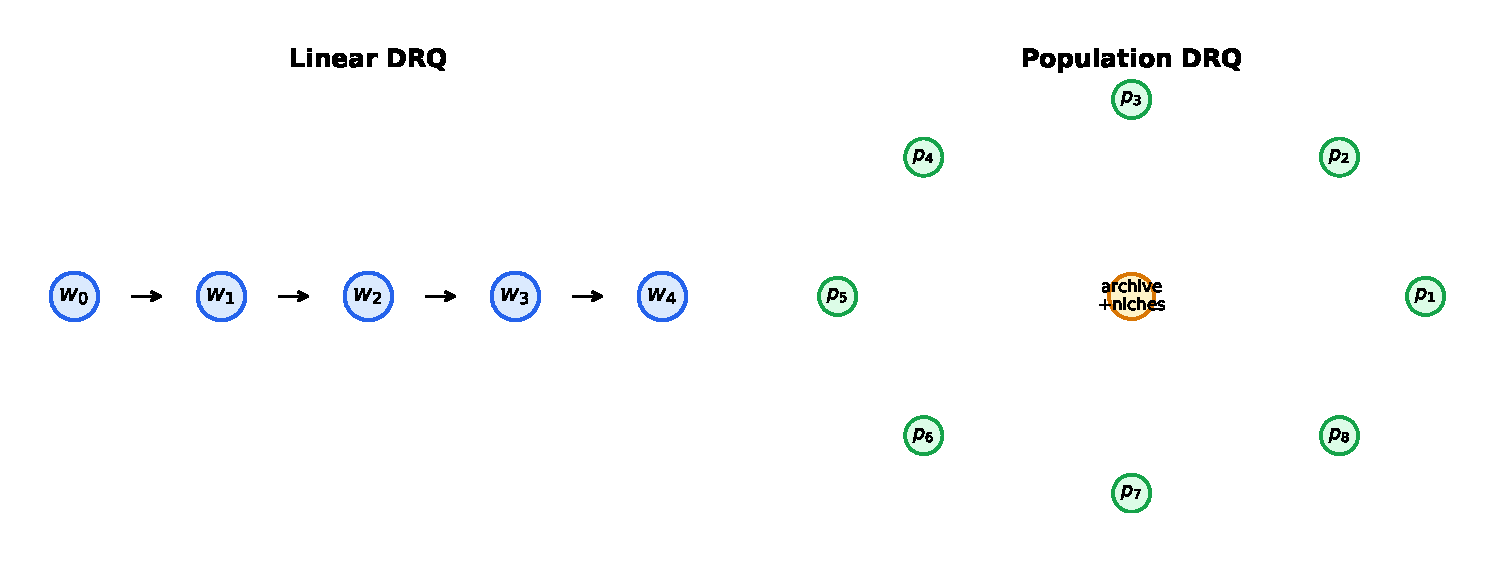
\includegraphics[width=\linewidth]{figures/fig_algorithm_diagram.pdf}
\caption{Linear DRQ optimizes a single sequence of champions against a growing archive. Population DRQ maintains simultaneous lineages, samples ecological tournaments, and uses replacement rules that can preserve specialists, novelty, and historical robustness.}
\label{fig:algorithm}
\end{figure}

\subsection{Algorithm family}

PDRQ is a family of related population models rather than a single fixed algorithm. We define six variants.

\paragraph{Linear DRQ baseline.}
The original method: one new champion is selected per round against all previous champions \citep{kumar2026digital}.

\paragraph{Population DRQ.}
A fixed-size population is updated by generating candidates from selected parents and testing them against sampled live opponents. Replacement removes ecologically weak individuals.

\paragraph{Population DRQ + archive.}
Opponents are sampled from both the live population and a historical archive. Archive pressure reduces forgetting but may bias the system toward generalists.

\paragraph{Population DRQ + novelty.}
Selection adds a novelty term computed from execution-trace descriptors, source embeddings, or static features. This tests whether diversity survives when it is explicitly rewarded.

\paragraph{Population DRQ + ecological persistence.}
Warriors receive credit for remaining viable across generations, not merely winning a single insertion tournament. This distinguishes durable niches from transient lucky counters.

\paragraph{Population DRQ + niche protection.}
Replacement is constrained by behavioral clusters so distinct strategy families retain representation. This tests whether ecological richness requires explicit protection or emerges from frequency-dependent selection alone.

\section{Finite-Game Theory}
\label{sec:finite_game_theory}

The main empirical question concerns LLM-generated Core War programs, but the reason to expect a difference between linear and population DRQ is already visible in finite games. Let $S=\{1,\ldots,n\}$ be a finite set of strategies and let $U\in[-1,1]^{n\times n}$ be the payoff matrix, where $U_{ij}$ is the payoff of strategy $i$ against strategy $j$. A mixed population or deployment policy is a distribution $\mu\in\Delta(S)$, and the expected payoff of pure strategy $i$ against $\mu$ is $(U\mu)_i$. For zero-sum or antisymmetric games, the payoff of an opponent that chooses pure strategy $i$ against deployed mixture $\mu$ is also $\mathbf{e}_i^\top U\mu$ under this row-player convention. For general-sum games, the same definition should use a separate opponent-payoff matrix. In the zero-sum setting we use opponent exploitability
\[
\operatorname{Exploit}(\mu)=\max_{i\in S}\mathbf{e}_i^\top U\mu,
\]
where smaller values mean that no pure opponent has a large positive payoff against the deployed mixture. Equivalently, one may report worst-case value $-\operatorname{Exploit}(\mu)$ for the deployed side. PDRQ improves robustness only when its deployable object $\mu_t$ has lower exploitability, not merely because $P_t$ is more diverse.

Linear DRQ can be idealized as a best-response process against an archive distribution
\[
h_t = \frac{1}{t}\sum_{\tau<t}\delta_{c_\tau},
\qquad
c_t\in \operatorname*{arg\,max}_{i\in S} (U h_t)_i.
\]
The current champion state is the pure strategy $c_t$. The archive $A_t$ can also induce a deployable mixture $\mu_t=h_t$ if deployment over archive members is allowed. Population DRQ instead maintains a live distribution $p_t$ and inserts candidates according to a score such as
\[
F_t(i)=(U Q_t)_i+\lambda_N N_t(i)+\lambda_P R_t(i)+\lambda_B B_t(i),
\qquad
Q_t=(1-\alpha)p_t+\alpha h_t .
\]
The parameter $\alpha$ controls archive pressure. When $\alpha=0$, selection is driven by the current ecology. When $\alpha=1$, selection is driven entirely by history. The distinction is therefore not ``mixture versus no mixture'' in the abstract; it is live ecological replacement versus post-hoc historical averaging, and current-champion deployment versus portfolio deployment.

\paragraph{Theorem 1: dominant strategies erase the population advantage.}
Suppose there is a unique strict dominant strategy $d$ such that $U_{dj}>U_{ij}$ for every $i\neq d$ and every opponent $j$. Assume incumbent retention is allowed, $d$ is reachable or retained once found, accepted candidates are selected elitistically by payoff against $Q_t$, and population replacement removes a lower-scoring incumbent when one exists. Once $d$ appears, linear current-champion DRQ with elitist retention keeps $c_t=d$, and performance-only PDRQ cannot improve on a population containing $d$ asymptotically. If $d$ remains retained or reachable and every non-$d$ incumbent is eventually compared against it under the same payoff criterion, repeated elitist replacement drives the live population toward $d$.

\paragraph{Counterexample 1: finite candidate budgets can delay or prevent convergence.}
The previous statement is not a guarantee for small LLM budgets. If the generator draws candidates from $G(\cdot\mid\mathrm{context})$ and $G(d\mid\mathrm{context})=0$ for the visited contexts, neither linear DRQ nor PDRQ can discover $d$. If $G(d\mid\mathrm{context})>0$ but very small, convergence is only probabilistic and may be invisible at pilot scale.

\paragraph{Counterexample 2: non-transitive games separate champions from deployable portfolios.}
Consider the zero-sum rock-paper-scissors payoff matrix
\[
U =
\begin{bmatrix}
0 & -1 & 1\\
1 & 0 & -1\\
-1 & 1 & 0
\end{bmatrix}.
\]
No pure champion is robust: for every pure deployment $\delta_j$, $\operatorname{Exploit}(\delta_j)=1$. The uniform mixture $\mu^\star=(1/3,1/3,1/3)$ has $\mathbf{e}_i^\top U \mu^\star=0$ for every pure strategy $i$, so $\operatorname{Exploit}(\mu^\star)=0$. Thus any method that deploys only $c_t$ remains exploitable, while a method that deploys a live or archived mixture can remove the pure-strategy vulnerability.

\paragraph{Implication.}
Cyclic dominance is not noise to be averaged away. In a non-transitive adversarial ecology, portfolio deployment is part of the solution. A linear DRQ sequence can reveal a cycle after the fact, and an archive-deployable linear DRQ can sometimes deploy a useful historical mixture. PDRQ's stronger claim is that live ecological replacement can maintain and adapt the mixture during search rather than reconstructing it only after the run.

\paragraph{Theorem 2: specialist value depends on deployment information.}
Let the evaluation environment contain two opponent classes, $x$ and $y$. Specialist $s_x$ scores $1$ against $x$ and $-1$ against $y$; specialist $s_y$ scores $-1$ against $x$ and $1$ against $y$; generalist $g$ scores $\epsilon$ against both, with $0<\epsilon<1$. Against a balanced archive-average objective, both specialists have average payoff $0$, while $g$ has payoff $\epsilon$, so archive-average selection prefers $g$. Under oracle portfolio selection, $\max\{u(s_x,x),u(s_y,x)\}=\max\{u(s_x,y),u(s_y,y)\}=1$, so the specialist pair dominates $g$. Under adaptive deployment with reliable opponent identification, choosing $s_x$ against $x$ and $s_y$ against $y$ also dominates $g$.

\paragraph{Counterexample 3: blind mixtures can lose to a generalist.}
If deployment is the blind uniform mixture over $\{s_x,s_y\}$, its expected payoff is $0$ against both opponent classes. The generalist $g$ scores $\epsilon>0$ against both and is strictly better. Thus specialist coexistence is not automatically robustness; the advantage appears under oracle selection, adaptive opponent identification, or a learned mixture that lowers exploitability relative to the generalist.

\paragraph{Implication.}
Full-history pressure can create robust generalists, but it can also hide specialist value. This is the central design tension in PDRQ: archive pressure prevents forgetting, while live-population pressure allows specialists to persist when their ecological target remains common.

\paragraph{Theorem 3: niche protection preserves support.}
Let $\phi:S\rightarrow\mathbb{R}^d$ be a descriptor map and let $\mathcal{N}=\{N_1,\ldots,N_k\}$ be a partition of $S$ into niches. Suppose each niche is occupied in $P_0$, and replacement is constrained so that a candidate in niche $N_m$ can replace only an incumbent from $P_t\cap N_m$. Then niche support is invariant: if $P_t\cap N_m\neq\varnothing$ for all $m$, then $P_{t+1}\cap N_m\neq\varnothing$ for all $m$. By contrast, unconstrained weakest-removal can collapse support in one insertion: if $a,b$ occupy distinct niches and a near-duplicate $a'\in N(a)$ has slightly higher score than $b$, weakest-removal replaces $b$ with $a'$, eliminating $N(b)$ from the live population.

\paragraph{Implication.}
The relevant empirical question is not only whether PDRQ maintains more programs, but whether replacement rules alter the reachable attractors of the adversarial process. The Core War experiment below tests the first measurable consequence of that possibility: whether archive+niche pressure changes the quality of the best warrior found under a matched LLM-call budget.

\paragraph{Finite-budget caveat.}
All claims above separate oracle dynamics from implementable DRQ. In the oracle model, $C_t$ contains the relevant best response or niche candidate. In the stochastic model, $C_t=\{c_1,\ldots,c_B\}$ with $c_b\sim G(\cdot\mid P_t,A_t,\mathrm{context})$, so a strategy matters only if it has positive reachability probability under visited contexts. With finite $B$, results hold in expectation or with high probability only after enough draws; with zero reachability, the formal game-theoretic optimum is operationally irrelevant.

\section{Implementation Design}

The implementation has four separable interfaces.

\paragraph{Evaluator.}
The evaluator compiles warriors, runs sampled tournaments under multiple offsets and rounds, and records win/loss/tie outcomes. For Core War, our implementation wraps pMARS and stores every warrior source file with a content hash.

\paragraph{Generator.}
The LLM generator receives parent source, opponent source or summaries, recent tournament failures, and constraints such as Redcode dialect, maximum length, and forbidden undefined behavior. It returns candidate source plus a short self-description. Invalid candidates count against the LLM-call budget.

\paragraph{Ecology manager.}
The manager maintains $P_t$, $A_t$, behavioral descriptors, lineage metadata, and replacement decisions. The Core War harness logs generated programs, completions, sampled opponents, and final summaries for every completed run.

\paragraph{Analysis pipeline.}
The analysis code computes generalization, diversity, cluster composition, payoff matrices, lineage trees, archive-forgetting curves, cross-run convergence, and predictive probes where the corresponding artifacts are available.

The repository accompanying this draft implements lightweight versions of these abstractions over a toy strategic ecology, together with the paid Core War harness used for the experiment. The toy ecology uses Core War-like role labels and an explicitly non-transitive payoff matrix, but it is not a Redcode interpreter and is not evidence that LLM-generated Core War populations behave this way. Its purpose is to make the population dynamics, metrics, and figure pipeline executable without paid LLM calls.

\section{Measurement Framework}

The empirical study below uses two headline metrics: mean final-population performance and best-champion performance. The broader PDRQ framework also motivates additional ecological measurements that are useful for future runs and for interpreting population behavior.

\paragraph{Generality.}
For warrior $w$ and held-out set $H$, generality is $\frac{1}{|H|}\sum_{h\in H}u(w,h)$ with confidence intervals over evaluator seeds. Worst-case generality reports $\min_{h\in H}u(w,h)$.

\paragraph{Portfolio robustness.}
For population $P$, oracle portfolio score is $\frac{1}{|H|}\sum_{h\in H}\max_{w\in P}u(w,h)$ and should be labeled as an upper bound when opponent identity is unavailable. Blind deployment evaluates a fixed mixture, such as the uniform distribution over $P$ or over $A_t$. Adaptive deployment first identifies an opponent cluster and then selects a warrior or mixture conditioned on that estimate. For a finite held-out opponent set $H$, empirical exploitability can be reported as $\widehat{\operatorname{Exploit}}_H(\mu)=\max_{h\in H}u(h,\mu)$, with lower values indicating better worst-case robustness.

\paragraph{Behavioral diversity.}
Diversity is the mean pairwise distance between normalized behavior descriptors. Entropy over discovered clusters reports population composition. Cluster persistence is the number of generations a cluster remains represented above a minimum frequency.

\paragraph{Ecological turnover.}
Turnover measures replacement rate, extinction count, re-emergence count, and mean lineage lifetime. Dominance turnover measures changes in the leading strategy cluster over time.

\paragraph{Non-transitivity.}
Cluster-level payoff matrices reveal cyclic dominance. A cycle score can be computed as the fraction of cluster triples $(a,b,c)$ where $a$ beats $b$, $b$ beats $c$, and $c$ beats $a$.

\section{Core War Experiment}

The finite-game analysis motivates PDRQ, but it does not establish that LLM-generated Redcode will enter the same regimes. We therefore ran a matched-budget Core War experiment designed to separate two distinct claims. The first is a population-quality claim: PDRQ might improve the average quality of the maintained final population. The second is a search claim: archive and niche pressure might improve the chance of finding one high-performing champion, even if the rest of the final population is mixed. The experiment supports the search claim but not the population-quality claim.

\subsection{Experimental configuration}

We compared three conditions. \emph{Linear DRQ} maintains a single champion selected against sampled historical opponents. \emph{Population current} maintains a live population of six warriors and evaluates candidates against sampled current-population opponents. \emph{Population archive+niche} also maintains a live population of six warriors, but mixes current opponents with archived opponents and uses a niche-aware replacement rule based on dominant opcode families. All three conditions used the same LLM-call budget, evaluator settings, held-out suite, candidate constraints, and invalid-generation handling.

The generator was Gemini 2.5 Flash through Vertex AI. Each long-profile replicate used 12 generations, 40 candidate generations per condition per generation, and three conditions, for a maximum of 1440 LLM calls per replicate. Candidate source length, prompt template, decoding settings, minimum instruction count, invalid-output threshold, opponent sampling, and held-out evaluation were fixed across conditions. Invalid candidates counted against the call budget.

All matches used pMARS v0.9.4, server build, with ICWS'94 extensions. The exact command template was
\[
\texttt{pmars -b -k -F <offset> -r 20 -s 8000 -c 80000 -p 8000 -l 100 -d 100 red blue}.
\]
Thus the Redcode dialect was pMARS ICWS'94, the core size was 8000, the cycle limit was 80000, the process limit was 8000, the maximum warrior length was 100, the minimum warrior distance was 100, the round count was 20, and the fixed offsets were 100, 500, and 1500. We did not pass an explicit P-space size; pMARS therefore used its default. Candidate validation used \texttt{pmars -A -b}, which assembles the warrior and evaluates \texttt{;assert} constraints. The seed corpus contained six starter warriors and the internal held-out corpus contained six warriors not used as initial seeds.

We report the 40 long-profile replicates used for the final analysis. These came from three batches: an initial 10-seed long run, a 20-seed verification run, and a final 10-seed verification run. Retries were assigned fresh run identifiers; partial failed attempts were retained for audit but excluded from aggregation unless they produced a completed summary. The estimated completed LLM cost for the 40 long-profile replicates was \$49.56.

\subsection{External Core War benchmarks}

Because the internal held-out suite is intentionally small, we added a second evaluation tier for Core War readers. We mirrored JKW's Wilkies benchmark from KOTH,\footnote{\url{http://www.koth.org/wilkies/}} the WilMoo benchmark from KOTH,\footnote{\url{http://www.koth.org/wilmoo/}} the Koenigstuhl 94nop Top-50 archive and full 94nop archive,\footnote{\url{https://asdflkj.net/COREWAR/koenigstuhl.html}} and the Corewar Global Masters 1 round 1 benchmark.\footnote{\url{https://corewar.co.uk/cgm1.htm}} The Koenigstuhl page explicitly recommends the Top-50 of the 94nop Koenigstuhl as a benchmark and describes the 94nop hill as standard core size 8000 with no P-space and no '88 programs.

These external evaluations are not official hill submissions and should not be read as Koenigstuhl rankings. They are fixed-setting replay checks under the same pMARS configuration used for the experiment. The current local benchmark set contains 12 Wilkies warriors, 12 WilMoo warriors, 60 warriors from the downloaded 94nop Top-50 archive, 20 CGM1 warriors, and a deterministic 50-warrior valid sample from the full Koenigstuhl 94nop archive. All imported benchmark warriors were assembled under the local pMARS binary before scoring.

\subsection{Core War validity checks}

All reported generated champions assemble under pMARS with ICWS'94 extensions. Invalid LLM generations were counted against the generation budget and discarded before tournament scoring. The evaluation used three fixed offsets rather than a single placement, reducing accidental dependence on one start distance, but it is still not a full official hill protocol and does not prove stability across all placements. We did not find evidence that the generated champions rely on P-space, non-assembling code, or dialect mismatch; none of the listed generated champions uses \texttt{ldp} or \texttt{stp}. The stronger caveat is overfitting: success on the six-warrior internal suite does not imply competitive strength against broader Core War corpora.

\subsection{Metrics}

We distinguish mean final-population performance from best-champion performance. For a population method, mean final-population performance is the average held-out score of the six final live population members. Best-champion performance is the held-out score of the strongest final warrior in that condition. For linear DRQ, these metrics are identical because the method returns a single champion. Unless otherwise stated, scores are normalized pMARS \texttt{-k} margins, computed as $(\mathrm{red}-\mathrm{blue})/(|\mathrm{red}|+|\mathrm{blue}|)$ from the two KOTH-style score rows emitted by pMARS. This is convenient for paired statistical analysis, but it should not be confused with an official hill rank or submission score.

This distinction is central. A population can be useful as a search process even if not every surviving member is strong. Conversely, a method that produces one excellent champion does not necessarily produce a robust deployable population. We therefore treat best-champion performance as the primary metric for the champion-discovery claim and mean final-population performance as the metric for broad population quality.

\subsection{Results}

\begin{table}[t]
\centering
\caption{Core War long-profile results across 40 paired seeds. Values are means $\pm$ approximate 95\% confidence intervals over seeds. ``Mean wins'' counts the number of seeds where a method had the highest mean final-population score. ``Best wins'' counts the number of seeds where a method had the highest best-champion score.}
\label{tab:corewar_long}
\begin{tabular}{lrrrr}
\toprule
Method & Mean population & Best champion & Mean wins & Best wins \\
\midrule
Linear DRQ & 0.4835$\pm$0.0355 & 0.4835$\pm$0.0355 & 19/40 & 10/40 \\
Population current & 0.4355$\pm$0.0499 & 0.4889$\pm$0.0479 & 10/40 & 10/40 \\
Population archive+niche & 0.4492$\pm$0.0328 & \textbf{0.5498$\pm$0.0370} & 11/40 & \textbf{20/40} \\
\bottomrule
\end{tabular}

\end{table}

\begin{table}[t]
\centering
\caption{External benchmark check for the eight highest-scoring generated champions by internal held-out score. Scores are mean normalized pMARS margins under the paper's fixed settings; negative values mean the generated warrior loses on average to the benchmark suite. K-Top50 denotes the downloaded Koenigstuhl 94nop Top-50 archive, Rand50 is a deterministic valid sample from the full 94nop archive, and CGM1 is the Corewar Global Masters round 1 benchmark.}
\label{tab:corewar_benchmarks}
\resizebox{\linewidth}{!}{\begin{tabular}{llrrrrrrrl}
\toprule
Warrior & Cond. & Len. & Internal & Wilkies & WilMoo & K-Top50 & Rand50 & CGM1 & Archetype \\
\midrule
current\_g007\_c0245\_bf8bf3df & current & 22 & 0.844 & -0.541 & -0.636 & -0.753 & -0.457 & -0.543 & stone/clear \\
current\_g001\_c0017\_67265a48 & current & 9 & 0.774 & -0.439 & -0.500 & -0.635 & -0.387 & -0.403 & paper/silk \\
archive\_g009\_c0359\_2352dfee & archive & 13 & 0.734 & -0.537 & -0.640 & -0.653 & -0.459 & -0.470 & vampire \\
archive\_g008\_c0320\_94b48fa8 & archive & 17 & 0.724 & -0.499 & -0.751 & -0.645 & -0.436 & -0.441 & vampire \\
current\_g011\_c0435\_1a64f14c & current & 14 & 0.715 & -0.528 & -0.742 & -0.741 & -0.465 & -0.520 & spl-based hybrid \\
archive\_g012\_c0453\_2529b8ee & archive & 12 & 0.709 & -0.412 & -0.437 & -0.356 & -0.250 & -0.280 & vampire \\
current\_g007\_c0264\_e18a383e & current & 20 & 0.706 & -0.551 & -0.760 & -0.774 & -0.513 & -0.492 & imp/imp-ring \\
archive\_g012\_c0470\_92d76e76 & archive & 6 & 0.689 & -0.648 & -0.751 & -0.839 & -0.587 & -0.651 & vampire \\
\bottomrule
\end{tabular}
}
\end{table}

Table~\ref{tab:corewar_long} shows the central empirical result. Linear DRQ has the highest observed mean final-population score: 0.4835 versus 0.4492 for archive+niche and 0.4355 for current-population PDRQ. Archive+niche therefore does not show a reliable population-mean advantage. In paired comparisons, archive+niche minus linear has mean difference $-0.0343$ with an approximate 95\% interval of $\pm 0.0565$, and archive+niche minus current has mean difference $0.0138$ with interval $\pm 0.0546$. Both intervals cross zero.

The best-champion metric tells a different story. Archive+niche has the highest average best-champion score, 0.5498, compared with 0.4889 for current-population PDRQ and 0.4835 for linear DRQ. In paired comparisons, archive+niche exceeds linear by $0.0663$ held-out score on average, with an approximate 95\% interval of $\pm 0.0584$ and normal-approximation $p\approx0.026$. Archive+niche exceeds current-population PDRQ by $0.0609$, with interval $\pm 0.0523$ and $p\approx0.022$. In nonparametric bootstrap resampling over paired seeds, archive+niche has the highest mean best-champion score among the three methods in 97.7\% of resamples.

Winner counts are consistent with this interpretation but less decisive on their own. Archive+niche wins best champion in 20 of 40 seeds, while linear and current-population each win 10. Against each single baseline, archive wins 25 of 40 paired seeds, so a simple sign test is not strong by itself. The evidence comes mainly from the size and consistency of the paired best-champion score advantage, not from a claim that archive+niche wins nearly every seed.

Table~\ref{tab:corewar_benchmarks} is the Core War credibility check. The top generated champions do not look hill-competitive under external benchmarks. The best internal champion scores 0.844 on the six-warrior internal held-out suite but $-0.541$ on Wilkies and $-0.753$ on the Koenigstuhl 94nop Top-50 replay. Every listed generated champion has negative mean margin against Wilkies, WilMoo, and Koenigstuhl Top-50. The nearest-source audit also shows that some high internal scorers are close to simple known archetypes rather than novel elite warriors; for example, the second-listed champion is nearest to the seed \texttt{paper} at 0.942 source similarity. A deterministic no-LLM template-bomber baseline selected from 50 variants scores 0.506 internally but also loses externally, with Wilkies $-0.687$, WilMoo $-0.644$, and Koenigstuhl Top-50 $-0.699$. Thus the LLM is doing meaningful search relative to the small internal task, but the generated warriors are not competitive Core War artifacts by current benchmark standards.

For trace-level inspection, we exported two pMARS score examples under \path{results/corewar_benchmarks/battle_examples}: the top internal champion beats \texttt{dwarf} 20--0 at offset 100 but loses 20--0 to \texttt{The Collective} at the same offset. These traces are intentionally modest: they show concrete behavior differences but are not a substitute for full hill-style benchmarking.

\subsection{Interpretation}

The experiment supports a narrower and more useful claim than broad population superiority. Archive+niche pressure appears to improve \emph{champion discovery}: it raises the expected quality of the best individual found during a run. It does not improve the average quality of all final live population members. This is the distinction predicted by the finite-game specialist analysis. Archive and niche pressure can preserve unusual candidates long enough to find a strong outlier, while the final population may still contain weaker specialists or artifacts of the training opponent distribution.

This result also explains why early batches appeared stronger than the final aggregate. The first 10 long seeds showed archive+niche winning best champion in 9 of 10 runs, but the 20-seed verification batch was much flatter. After 40 paired seeds, the conclusion is measured: archive+niche is useful as a search-diversification mechanism, not as a generally superior population optimizer. Separately, the external benchmark check shows that the generated champions should not yet be presented as competitive warriors. The scientific result is about search dynamics inside a controlled LLM experiment; competitive Core War strength would require much broader training and validation.

\section{Controlled Surrogate Study}

The repository includes an executable toy ecology with six strategic roles: bomber, scanner, replicator, anti-scanner, defender, and hybrid. The payoff matrix is deliberately non-transitive, and the mutation operator is a hand-coded proxy for semantic LLM mutation. This surrogate is best read as a controlled demonstration of the theory in Section~\ref{sec:finite_game_theory}: when the world contains non-transitive roles, population methods can preserve complementary strategies and produce portfolio gains that a single champion cannot. It does not validate claims about LLM-generated Core War warriors.

\begin{table}[t]
\centering
\caption{Toy surrogate results from the default controlled run. Values are means $\pm$ standard errors across seeds. These numbers demonstrate the synthetic non-transitive ecology and should not be interpreted as Core War results.}
\label{tab:pilot}
% Generated from 4 surrogate seeds by experiments/run_toy_ecology.py
\begin{tabular}{lrrrr}
\toprule
Method & Best held-out & Oracle portfolio & Diversity & Role entropy \\
\midrule
Static opponent & 0.112$\pm$0.001 & 0.112$\pm$0.001 & 0.000$\pm$0.000 & 0.000$\pm$0.000 \\
Linear DRQ & 0.049$\pm$0.038 & 0.049$\pm$0.038 & 0.000$\pm$0.000 & 0.000$\pm$0.000 \\
Population & 0.110$\pm$0.002 & 0.315$\pm$0.004 & 1.263$\pm$0.025 & 1.994$\pm$0.052 \\
Population + archive & 0.107$\pm$0.001 & 0.321$\pm$0.004 & 1.279$\pm$0.021 & 2.221$\pm$0.057 \\
Population + novelty & 0.105$\pm$0.005 & 0.328$\pm$0.001 & 1.400$\pm$0.009 & 2.475$\pm$0.026 \\
Population + niche & 0.110$\pm$0.002 & 0.324$\pm$0.001 & 1.310$\pm$0.036 & 2.192$\pm$0.103 \\
\bottomrule
\end{tabular}

\end{table}

\begin{figure}[t]
\centering
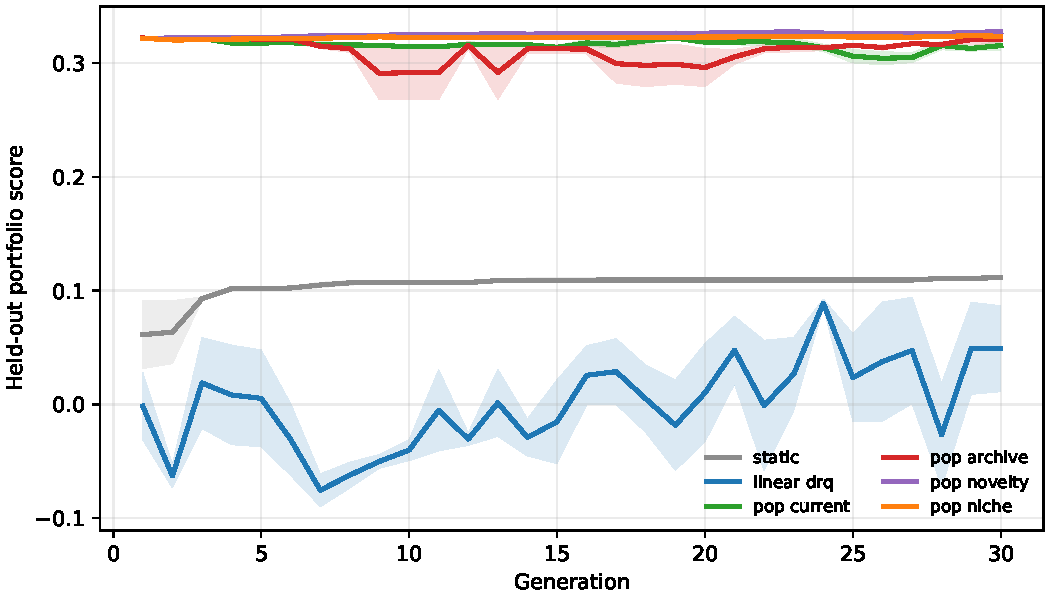
\includegraphics[width=0.95\linewidth]{figures/fig_pilot_performance.pdf}
\caption{Surrogate held-out portfolio score over generations. In this controlled non-transitive ecology, population variants can preserve complementary roles that improve oracle portfolio score.}
\label{fig:performance}
\end{figure}

\begin{figure}[t]
\centering
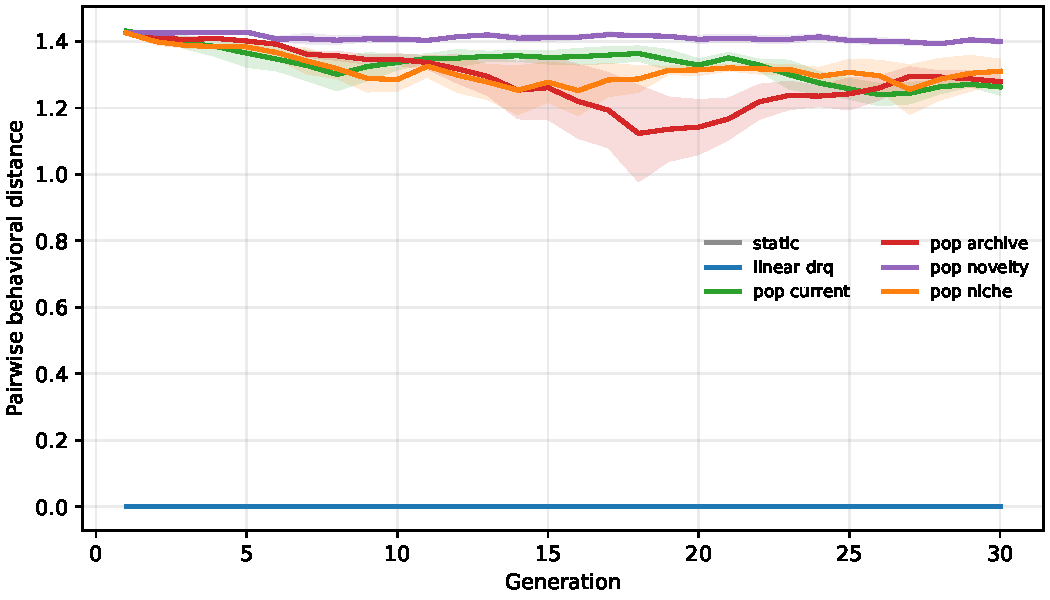
\includegraphics[width=0.95\linewidth]{figures/fig_pilot_diversity.pdf}
\caption{Surrogate behavioral diversity over generations. Single-champion baselines have zero within-population diversity by definition, while population variants expose how replacement rules alter diversity.}
\label{fig:diversity}
\end{figure}

\begin{figure}[t]
\centering
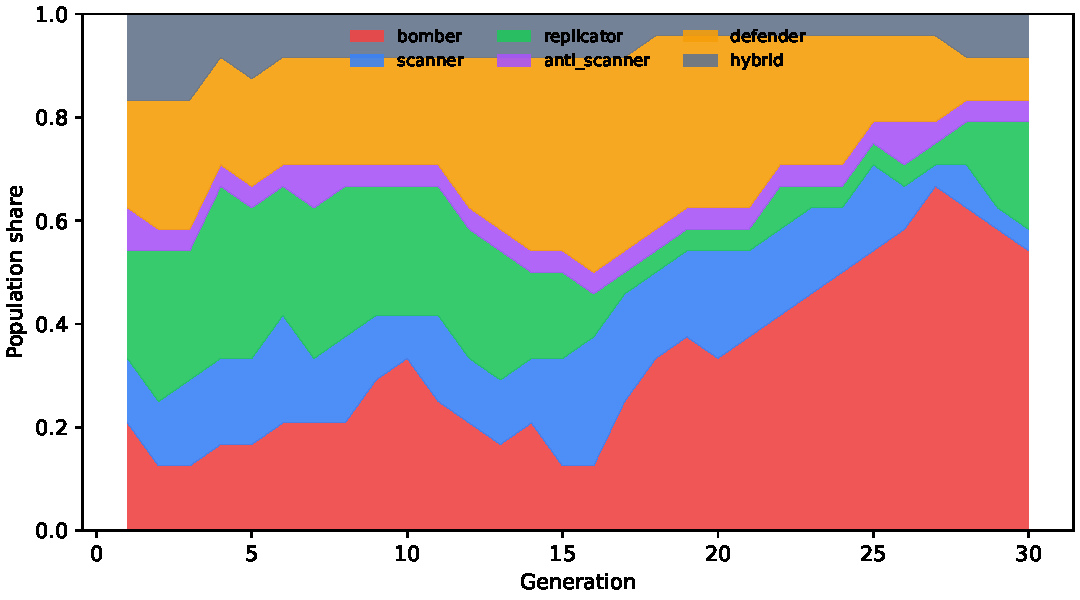
\includegraphics[width=0.95\linewidth]{figures/fig_pilot_composition.pdf}
\caption{Example surrogate population composition time series for the niche-protected variant. A richer Core War analysis would replace synthetic roles with clusters derived from execution traces.}
\label{fig:composition}
\end{figure}

\begin{figure}[t]
\centering
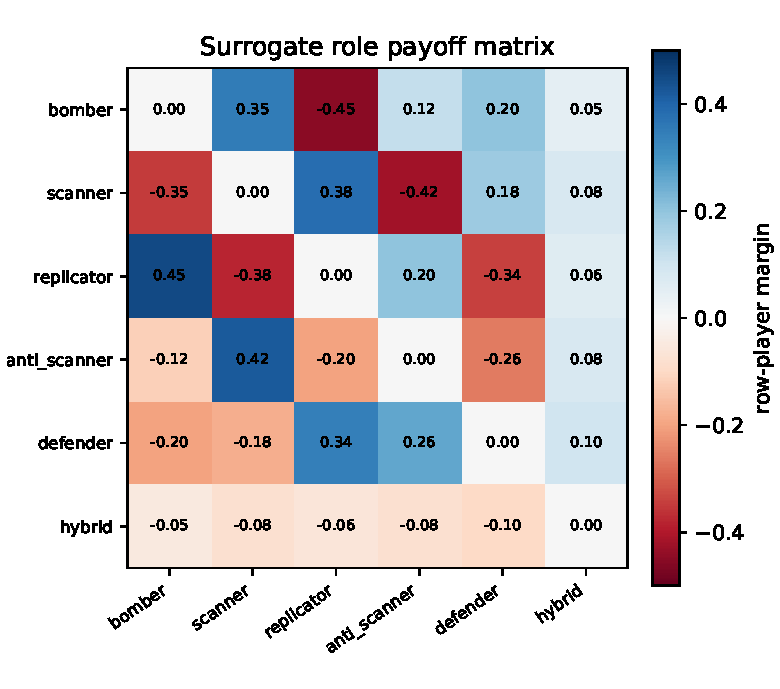
\includegraphics[width=0.72\linewidth]{figures/fig_payoff_matrix.pdf}
\caption{Surrogate role payoff matrix. The matrix is hand-designed to contain non-transitive structure, so it demonstrates measurement behavior rather than discovering Core War ecology.}
\label{fig:payoff}
\end{figure}

\begin{figure}[t]
\centering
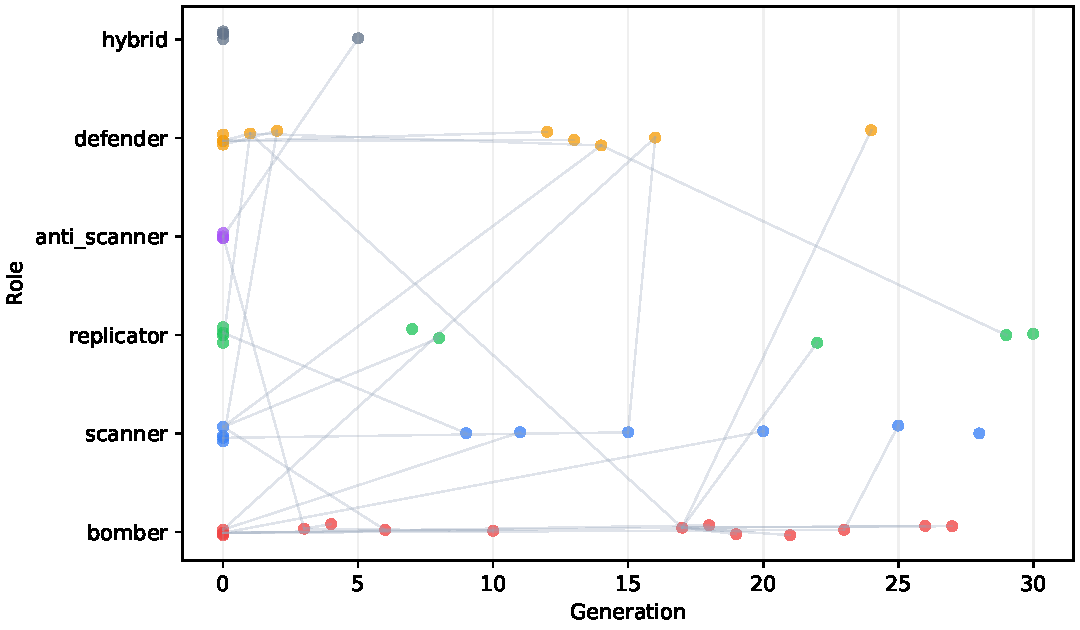
\includegraphics[width=0.95\linewidth]{figures/fig_lineage_tree.pdf}
\caption{Surrogate lineage tree for accepted warriors. Core War lineage analysis should use source hashes and parent prompts to reconstruct ancestry.}
\label{fig:lineage}
\end{figure}

\begin{figure}[t]
\centering
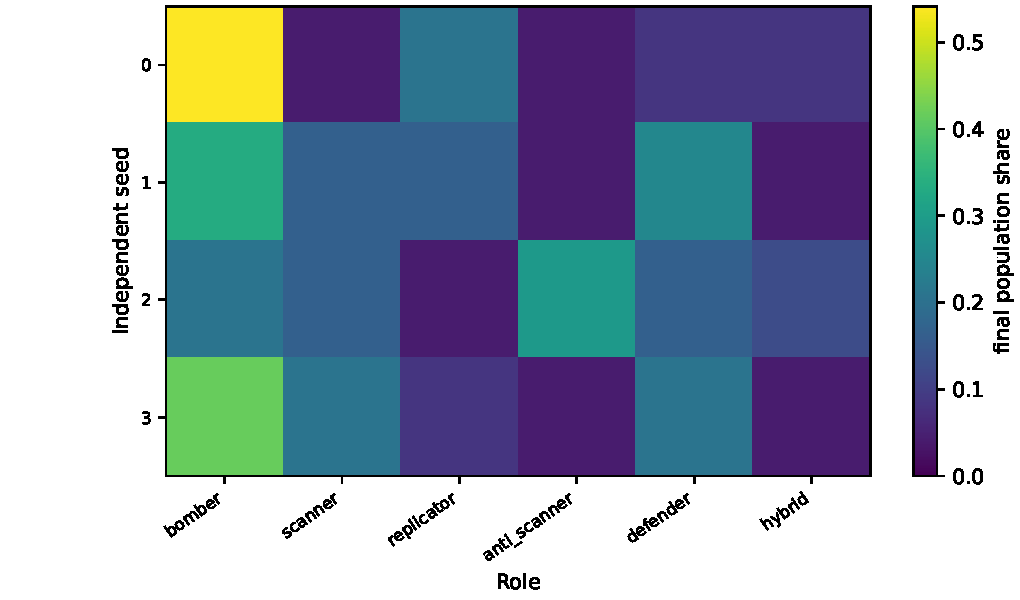
\includegraphics[width=0.85\linewidth]{figures/fig_cross_run_roles.pdf}
\caption{Cross-run surrogate final role composition. In Core War, the analogous question is whether independently evolved populations converge to similar behavioral roles rather than identical source code.}
\label{fig:crossrun}
\end{figure}

\begin{figure}[t]
\centering
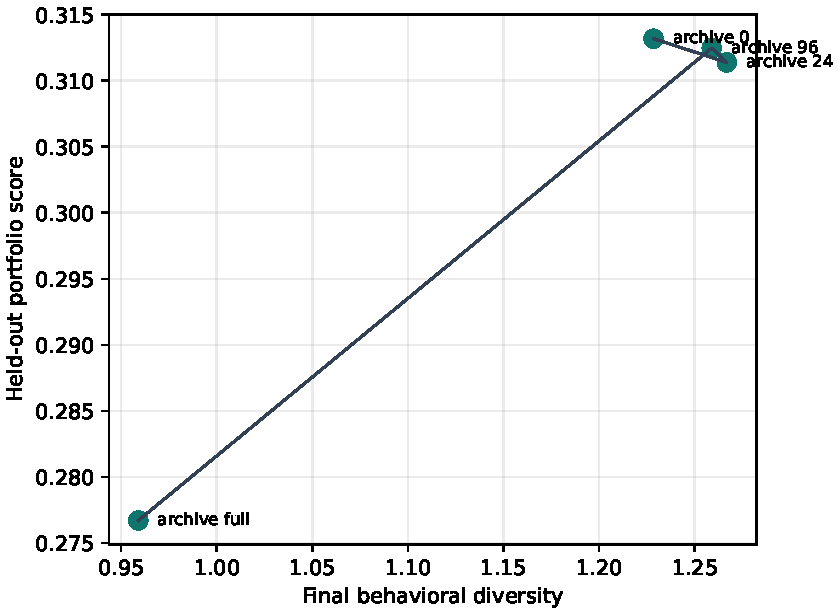
\includegraphics[width=0.78\linewidth]{figures/fig_archive_tradeoff.pdf}
\caption{Surrogate archive-size tradeoff between final diversity and held-out portfolio score. This plot illustrates the archive-pressure tension predicted by the finite-game analysis.}
\label{fig:archive}
\end{figure}

\begin{figure}[t]
\centering
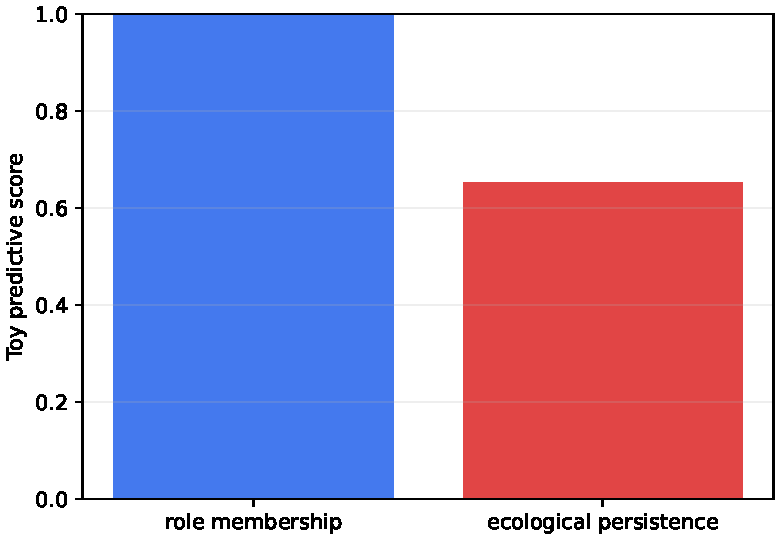
\includegraphics[width=0.70\linewidth]{figures/fig_predictive_pilot.pdf}
\caption{Surrogate predictive probes for role and persistence. In Core War, probes should use source embeddings, trace embeddings, and static program features.}
\label{fig:predictive}
\end{figure}

\section{Threats to Validity}

\paragraph{LLM stochasticity.}
LLM outputs depend on model version, decoding settings, prompt format, and safety filters. We logged prompts, completions, invalid generations, run IDs, and retries, but the experiment still samples a stochastic generator rather than a deterministic mutation distribution. The results should therefore be treated as estimates for this model, prompt, and date, not as universal properties of LLM-generated Core War.

\paragraph{Evaluator artifacts.}
Core War outcomes can depend on MARS dialect, core size, initialization distance, maximum cycles, process limits, maximum warrior length, P-space settings, and seed schedule. We fixed pMARS and used a fixed offset and round schedule, but we did not run official Koenigstuhl or KOTH submission protocols. The 94nop replay is therefore a benchmark-style sanity check, not a claim of 94nop hill equivalence. Robustness across hill settings remains open.

\paragraph{Descriptor validity.}
The archive+niche condition used a simple niche proxy based on dominant opcode families. This is useful for a first experiment, but it is not a full behavioral descriptor. Source similarity, trace similarity, payoff similarity, and dynamic execution features should be analyzed separately before making strong ecological claims.

\paragraph{Budget fairness.}
The main comparison matched LLM calls across conditions, counted invalid generations against the budget, and reported completed estimated cost. Population methods still maintain more live state than linear DRQ, so there may be additional bookkeeping and evaluator costs not captured by LLM-call parity alone.

\paragraph{Portfolio evaluation.}
The present empirical claim is about best-champion discovery, not deployable portfolio robustness. Oracle portfolio selection can overstate deployable robustness, and we do not claim that the final archive+niche population is itself a better deployment policy. Fixed mixtures, learned mixtures, and adaptive opponent-identification settings remain future work.

\paragraph{Competitive Core War strength.}
The external benchmark replay shows that the generated champions are not competitive with established human-written benchmark warriors. This is a limitation of the current experiment, but it also protects the main claim from overreach: PDRQ improved search inside the small controlled suite, not Core War hill performance. A version aimed primarily at the Core War community should treat external benchmark strength as the main competitive yardstick and the six-warrior held-out suite as an internal search diagnostic.

\paragraph{Surrogate limitations.}
The included toy ecology has hand-designed roles and payoff cycles. It illustrates the finite-game argument and validates implementation mechanics, but it cannot answer whether LLM-generated Core War warriors form comparable ecological roles.

\section{Discussion}

Population DRQ reframes LLM-driven program evolution from a search for one better program into a model of adversarial ecosystems. This matters scientifically because non-transitive games often do not have a single best strategy. It matters practically because domains such as automated red-teaming and cybersecurity involve changing populations of attacks and defenses. The Core War result shows both the promise and the limit of this framing. Population structure helped the search find higher-scoring champions on the internal task, but it did not make the maintained population better on average, did not establish a deployable portfolio, and did not produce externally competitive warriors.

The key design tension is archive pressure. Historical archives stabilize learning and prevent forgetting, but full archives may convert ecology back into static generalist optimization. Current-population training leaves more room for cycling and specialist niches, but may forget old vulnerabilities. Niche protection can preserve unusual candidates, but preservation alone is not the goal: the candidates must either improve deployable robustness or improve search by uncovering stronger champions. In the experiment reported here, the evidence favors the second interpretation.

The finite-game analysis shows why these mechanisms can matter, and the controlled surrogate demonstrates the same distinctions in an executable setting. The Core War experiment then tests one concrete transfer to real LLM-generated Redcode. The result is not a full ecological validation: we have not shown stable payoff cycles, persistent behavioral niches, deployable mixture robustness, or hill competitiveness. But it does show that archive+niche pressure can improve best-champion discovery under a matched LLM budget. That is a meaningful, narrower empirical contribution.

\section{Conclusion}

This paper proposes Population Digital Red Queen, a population-level extension of LLM-driven adversarial program evolution. The central theoretical point is that portfolio deployment can represent ecological states that a single current champion cannot, including mixed equilibria, persistent niches, cyclic dominance, turnover, branching ancestry, and portfolio robustness, and that live population replacement can maintain such states during search. We formalize that distinction in finite games, define an algorithm family for LLM-generated programs, provide metrics for ecological analysis, and release an executable surrogate scaffold.

The completed Core War study gives a qualified empirical result. Across 40 matched long-profile runs, archive+niche PDRQ does not improve mean final-population performance, but it does produce higher-scoring best champions on average than linear DRQ or current-population PDRQ. The conclusion is not that population DRQ dominates linear DRQ, nor that the generated warriors are competitive on established Core War benchmarks. It is that archive and niche pressure can be valuable as a search-diversification mechanism for discovering high-performing adversarial programs inside a controlled evaluation. Future work should test whether that champion-discovery advantage can be converted into deployable portfolio robustness and external benchmark strength through better descriptors, mixture policies, adaptive opponent identification, and larger human-warrior training corpora.

\appendix
\section{Generated Warrior Listings}
\label{app:generated_warriors}

The following listings show the highest-scoring generated champions by internal held-out score. Each listing includes the condition, run, internal score, external benchmark scores, heuristic archetype, source length, and nearest reference by source similarity. These programs are included for inspection; the external benchmark results in Table~\ref{tab:corewar_benchmarks} show that they are not hill-competitive. Source comments are line-wrapped for print; exact executable files are exported under \texttt{results/corewar\_benchmarks/champions}.

% Generated by experiments/benchmark_corewar_champions.py
\subsection*{Generated warrior 1: pop\_current\_g007\_c0245\_bf8bf3df}
\begin{description}
\item[Condition] pop\_current
\item[Run] verify\_long\_20260515T171256Z\_long\_s2015\_a01, seed 2015
\item[Scores] internal 0.844; Wilkies -0.541; WilMoo -0.636; Koenigstuhl Top-50 -0.753
\item[Archetype] stone/clear; length 22; nearest reference dwarf (0.358)
\end{description}
\begingroup\small
\begin{verbatim}
;redcode-94
;assert 1
;name Hybrid Bomb Spreader 7.0
;author Generated
start   spl 0
        mov.i clear_val, <ptr_clear
        add #14, ptr
        mov bomb, @ptr
        add #21, ptr2
        mov bomb2, @ptr2
        add #28, ptr3
        mov bomb3, @ptr3
        add #35, ptr4
        mov bomb4, @ptr4
        add #42, ptr_clear
        jmp start
bomb    dat #0, #1
ptr     dat #0, #0
bomb2   dat #0, #2
ptr2    dat #0, #0
bomb3   dat #0, #3
ptr3    dat #0, #0
bomb4   dat #0, #4
ptr4    dat #0, #0
clear_val dat #0, #0
ptr_clear dat #0, #0
        end start
\end{verbatim}
\endgroup

\subsection*{Generated warrior 2: pop\_current\_g001\_c0017\_67265a48}
\begin{description}
\item[Condition] pop\_current
\item[Run] verify\_long\_extra10\_20260516T175027Z\_long\_s2026\_a01, seed 2026
\item[Scores] internal 0.774; Wilkies -0.439; WilMoo -0.500; Koenigstuhl Top-50 -0.635
\item[Archetype] paper/silk; length 9; nearest reference paper (0.942)
\end{description}
\begingroup\small
\begin{verbatim}
;redcode-94
;assert 1
;name PDRQ Modified Paper Splitter
;author PDRQ setup + mutation
; strategy a replicator that splits, with an attack at the end of
; the copy
        org start
start   spl copy
        spl 1
copy    mov <src, <dst
        djn copy, #6
        mov #1, @-1 ; Attack after replication
        jmp @dst
src     dat #0, #last
dst     dat #0, #150
last    dat #0, #0
        end start
\end{verbatim}
\endgroup

\subsection*{Generated warrior 3: pop\_archive\_niche\_g009\_c0359\_2352dfee}
\begin{description}
\item[Condition] pop\_archive\_niche
\item[Run] verify\_long\_20260515T171256Z\_long\_s2009\_a02, seed 2009
\item[Scores] internal 0.734; Wilkies -0.537; WilMoo -0.640; Koenigstuhl Top-50 -0.653
\item[Archetype] vampire; length 13; nearest reference vampire (0.648)
\end{description}
\begingroup\small
\begin{verbatim}
;redcode-94
;assert 1
; name PDRQ Stone Vampire Hunter v3.2 - Adaptive Split & Bomb
; (Recombined)
;author PDRQ setup / AI / Mutated / Recombined
; strategy A hybrid that splits, uses a vampire-like attack, and
; overwrites with DATs. Further increased adaptive splitting and
; bomb spread for wider coverage and disruption.
        org start
start   spl 0, <ptr_inc ; Adaptive initial split for wider
; coverage
        add #7, fang
        mov fang, @fang
        add #11, ptr ; Increased adaptive increment for bomb
; spread
        mov bomb, @ptr
        djn next, #99 ; More aggressive loop count for more bombs
; and splits
next    jmp start
fang    jmp trap, #100
trap    spl 0
        jmp trap
bomb    dat #0, #0
ptr     dat #0, #1
ptr_inc dat #0, #7       ; Adjusted adaptive split increment
        end start
\end{verbatim}
\endgroup

\subsection*{Generated warrior 4: pop\_archive\_niche\_g008\_c0320\_94b48fa8}
\begin{description}
\item[Condition] pop\_archive\_niche
\item[Run] scaleup\_flash\_20260515T052028Z\_long\_s1003\_a01, seed 1003
\item[Scores] internal 0.724; Wilkies -0.499; WilMoo -0.751; Koenigstuhl Top-50 -0.645
\item[Archetype] vampire; length 17; nearest reference paper (0.594)
\end{description}
\begingroup\small
\begin{verbatim}
;redcode-94
;assert 1
; name PDRQ Splitter Vampire Bomb Enhanced 9.1 (Fang and Bomb
; Spread Variation)
;author PDRQ setup
start   spl 0
        add #8, fang  ; Varied fang spread
        mov fang, @fang
        add #5, ptr   ; Varied bomb spacing
        mov bomb, @ptr
        spl copy
        jmp start
copy    mov <src, <dst
        djn copy, #7  ; Varied copy length
        jmp @dst
fang    jmp trap, #100
trap    spl 0
        jmp trap
bomb    dat #0, #0
src     dat #0, #0
dst     dat #0, #200
ptr     dat #0, #0
        end start
\end{verbatim}
\endgroup

\subsection*{Generated warrior 5: pop\_current\_g011\_c0435\_1a64f14c}
\begin{description}
\item[Condition] pop\_current
\item[Run] scaleup\_flash\_20260515T052028Z\_long\_s1008\_a01, seed 1008
\item[Scores] internal 0.715; Wilkies -0.528; WilMoo -0.742; Koenigstuhl Top-50 -0.741
\item[Archetype] spl-based hybrid; length 14; nearest reference paper (0.739)
\end{description}
\begingroup\small
\begin{verbatim}
;redcode-94
;assert 1
;name Rapid Spreader (Mutated)
;author AI
; strategy Focuses on rapid spreading and bombing, with a slightly
; smaller replication size for faster deployment.
        org start
start   spl copy        ; Start replication
        mov bomb, @ptr  ; Bomb an address pointed to by ptr
        add #5, ptr ; Increment ptr to bomb a new location
; (slightly slower bombing frequency)
        add #40, dst ; Dynamically adjust replication destination
; for wider spread
        spl 0, #5 ; Split, new process starts 5 instructions after
; this one for very fast spread
        jmp start       ; Loop back to bomb again
copy    mov <src, <dst  ; Replicate instructions
        djn copy, #12 ; Loop 12 times for replication (smaller
; replication size)
        jmp @dst        ; Jump to the replicated code
src     dat #0, #last   ; Source for replication
dst     dat #0, #200    ; Destination for replication
bomb    dat #0, #0      ; Bomb instruction
ptr     dat #0, #1      ; Pointer for bombing
last    dat #0, #0      ; End of replication source
        end start
\end{verbatim}
\endgroup

\subsection*{Generated warrior 6: pop\_archive\_niche\_g012\_c0453\_2529b8ee}
\begin{description}
\item[Condition] pop\_archive\_niche
\item[Run] verify\_long\_extra10\_20260516T175027Z\_long\_s2026\_a01, seed 2026
\item[Scores] internal 0.709; Wilkies -0.412; WilMoo -0.437; Koenigstuhl Top-50 -0.356
\item[Archetype] vampire; length 12; nearest reference vampire (0.523)
\end{description}
\begingroup\small
\begin{verbatim}
;redcode-94
;assert 1
; name PDRQ Hybrid Bomb-Vampire (Adaptive Spread, Dual Offset) -
; Optimized
;author PDRQ setup (Recombination) - Optimized
start   spl 0
        mov bomb, <bomb_target
        mov fang, @fang_target
        add #28, bomb_target ; Slightly increased bomb spread
        add #22, fang_target ; Slightly increased vampire spread
        jmp start
bomb    dat #0, #0
fang    jmp trap, #100
trap    spl -1
        jmp trap
bomb_target dat #0, #110 ; Adjusted initial offset
fang_target dat #0, #90  ; Adjusted initial offset
end start
\end{verbatim}
\endgroup

\subsection*{Generated warrior 7: pop\_current\_g007\_c0264\_e18a383e}
\begin{description}
\item[Condition] pop\_current
\item[Run] verify\_long\_20260515T171256Z\_long\_s2011\_a02, seed 2011
\item[Scores] internal 0.706; Wilkies -0.551; WilMoo -0.760; Koenigstuhl Top-50 -0.774
\item[Archetype] imp/imp-ring; length 20; nearest reference paper (0.613)
\end{description}
\begingroup\small
\begin{verbatim}
;redcode-94
;assert 1
; name PDRQ Seed Vampire - Mutation 18 (Aggressive, Wider, Faster,
; Quad Bomb, Anti-Paper)
;author PDRQ setup / AI
; strategy An even more aggressive fang bomber with wider spread,
; faster bombing, anti-paper, and self-replication for increased
; presence, with a quad bomb for enhanced attack.
        org start
start   spl copy      ; Start a self-replication process
        add #37, fang ; Wider spread to hit more areas quickly
        mov fang, @fang
        jmp start
copy    mov <src, <dst
        djn copy, #6  ; Replicate 6 instructions
        jmp @dst      ; Jump to the new copy
src     dat #0, #last
dst     dat #0, #300
last    dat #0, #0
        add #1, dst   ; Update destination for next copy
        mov dst, @dst
fang    jmp trap, #58 ; Faster bombing, more aggressive
trap    spl 0
        mov 0, 1      ; Small anti-paper modification
        mov #0, @-2   ; Dual bomb for enhanced attack
        mov #0, @-3   ; Triple bomb for enhanced attack
        mov #0, @-4   ; Quad bomb for enhanced attack
        mov -1, -1    ; Added for core robustness
        jmp trap
        end start
\end{verbatim}
\endgroup

\subsection*{Generated warrior 8: pop\_archive\_niche\_g012\_c0470\_92d76e76}
\begin{description}
\item[Condition] pop\_archive\_niche
\item[Run] scaleup\_flash\_20260515T052028Z\_long\_s1001\_a02, seed 1001
\item[Scores] internal 0.689; Wilkies -0.648; WilMoo -0.751; Koenigstuhl Top-50 -0.839
\item[Archetype] vampire; length 6; nearest reference vampire (0.656)
\end{description}
\begingroup\small
\begin{verbatim}
;redcode-94
;assert 1
;name Hybrid Dwarf Spread Faster (Aggressive Bomb Recomb)
;author PDRQ setup (modified)
start   spl 0
        add #1, fang
        mov bomb, @fang
        jmp -2
fang    jmp bomb, #10
bomb    mov 0, <0 ; Changed to MOV bomb for more aggressive
; killing
        end start
\end{verbatim}
\endgroup


\section{Reproducibility Artifact Checklist}
\label{app:artifacts}

The repository includes the following artifacts for reproducing the Core War checks.

\begin{itemize}
\item pMARS binary: \path{vendor/pmars-bin}; version checked as \texttt{pMARS v0.9.4, 04/07/22, corewar simulator with ICWS'94 extensions}.
\item Internal seed warriors: \path{data/corewar/seeds}.
\item Internal held-out warriors: \path{data/corewar/heldout}.
\item External benchmark manifest: \path{data/corewar/benchmarks/manifest.json}; mirrored suites are stored under \path{data/corewar/benchmarks}.
\item Generated champion files: \path{results/corewar_benchmarks/champions}.
\item Main external benchmark summary: \path{results/corewar_benchmarks/benchmark_results.json}.
\item Champion CSV summary: \path{results/corewar_benchmarks/champion_benchmark_summary.csv}.
\item No-LLM template baseline summary: \path{results/corewar_benchmarks/template_baseline.json}.
\item Battle examples: \path{results/corewar_benchmarks/battle_examples}.
\item Paper tables generated from benchmark artifacts: \path{paper/tables/corewar_benchmark_summary.tex} and \path{paper/tables/generated_warriors_appendix.tex}.
\end{itemize}

The external benchmark suite can be refreshed with:
\begin{verbatim}
python3 scripts/fetch_corewar_benchmarks.py
\end{verbatim}

The champion benchmark replay can be rerun with:
\begin{verbatim}
.venv/bin/python experiments/benchmark_corewar_champions.py \
  --top-n 10 \
  --match-rounds 20 \
  --match-timeout 3 \
  --offsets 100 500 1500
\end{verbatim}

The no-LLM template-mutator baseline can be rerun with:
\begin{verbatim}
.venv/bin/python experiments/run_corewar_template_baseline.py
\end{verbatim}

The combined target is:
\begin{verbatim}
make benchmark-corewar
\end{verbatim}

\bibliographystyle{plainnat}
\bibliography{references}

\end{document}
